\documentclass[conference]{IEEEtran}
\IEEEoverridecommandlockouts

\usepackage{cite}
\usepackage{amsmath,amssymb,amsfonts}
\usepackage{booktabs}
\usepackage{url}
\usepackage{graphicx}
\usepackage{tikz}
\usepackage{pgfplots}
\pgfplotsset{compat=1.18}
\usetikzlibrary{arrows.meta,positioning,shapes.geometric,calc}
% hyperref MUST be loaded LAST
\usepackage{hyperref}

\begin{document}

\title{Vision-Based Connect-4 Robot: Image Processing Pipeline\\
for Autonomous Game-State Extraction and Motor Control}

\author{%
\IEEEauthorblockN{Andrew Abdelmalak}
\IEEEauthorblockA{\textit{Dept.\ of Mechatronics Engineering}\\
\textit{German University in Cairo}\\
Cairo, Egypt\\
55-22771}
\and
\IEEEauthorblockN{Daniel Boules}
\IEEEauthorblockA{\textit{Dept.\ of Mechatronics Engineering}\\
\textit{German University in Cairo}\\
Cairo, Egypt\\
55-5055}
\and
\IEEEauthorblockN{David Girgis}
\IEEEauthorblockA{\textit{Dept.\ of Mechatronics Engineering}\\
\textit{German University in Cairo}\\
Cairo, Egypt\\
55-1481}
\and
\IEEEauthorblockN{Kirolous Kirolous}
\IEEEauthorblockA{\textit{Dept.\ of Mechatronics Engineering}\\
\textit{German University in Cairo}\\
Cairo, Egypt\\
55-18081}
\and
\IEEEauthorblockN{Samir Yacoub}
\IEEEauthorblockA{\textit{Dept.\ of Mechatronics Engineering}\\
\textit{German University in Cairo}\\
Cairo, Egypt\\
55-25111}
\and
\IEEEauthorblockN{Youssef Salama}
\IEEEauthorblockA{\textit{Dept.\ of Mechatronics Engineering}\\
\textit{German University in Cairo}\\
Cairo, Egypt\\
55-0540}
}

\maketitle

\begin{abstract}
Connect-4 is a two-player, zero-sum board game that provides a compact yet
demanding testbed for integrating computer vision, decision-making, and
robotic actuation within a single embedded loop. This paper describes a
Vision-Based Connect-4 Robot built on a Raspberry Pi~4 with a Pi Camera~V2
that captures overhead board frames and processes them through a
Python/OpenCV pipeline comprising geometric rotation, perspective warping,
brightness and contrast adjustment, Gaussian smoothing, and HSV-based cell
classification. The pipeline extracts a verified $6\times7$ game-state
matrix, which a trusted-state validator checks against six legality rules
before a minimax search with alpha-beta pruning at depth~5 selects the
robot's move. The chosen column is transmitted over a 9600-baud serial
link to an Arduino Uno that drives a TT carriage motor and an
encoder-coupled magazine motor through an L298N H-bridge, dispensing one
token into the selected column. The camera then re-reads the board to
verify that the move was executed correctly, closing the
perception-to-actuation loop. The HSV classifier achieved 98\% per-cell
accuracy, the magazine-to-column mechanism attained a 95\% overall drop
success rate, and the full system passed all 31 integration tests. These
results demonstrate that real-time vision, trusted-state validation, and
closed-loop physical actuation can be integrated on commodity embedded
hardware for autonomous game play.
\end{abstract}

\begin{IEEEkeywords}
connect-4 robot, image processing pipeline, HSV color segmentation, minimax algorithm, closed-loop verification
\end{IEEEkeywords}

% ===========================================================================
\section{Introduction}
% ===========================================================================

Autonomous game-playing robots are compelling mechatronic testbeds because
they demand tightly integrated perception, cognition, and actuation
operating in a real-time loop~\cite{Zubek2021}. Board games such as chess
and Connect-4 require a robot to acquire an image of the board, extract the
complete game state, reason about the optimal move, and physically execute
that move with repeatable accuracy---all within a time frame acceptable for
human--robot interaction. The open-source chess robot
in~\cite{Abarkan2024} demonstrated that a three-axis Cartesian gantry can
achieve $\pm 1.5$\,mm repeatability at 3\,s per move, while the modular
CNN chess-recognition pipeline in~\cite{Wolflein2021} achieved greater than
98\% per-square accuracy. Connect-4 offers a simpler mechanical
requirement---only a single horizontal axis is needed for column
selection---but adds the challenge of reliable two-color (red/yellow)
token classification under variable ambient lighting.

Connect-4 is a two-player, zero-sum game in which the first player to align
four same-colored discs horizontally, vertically, or diagonally wins. Tokens
fall under gravity once released above the correct column, which simplifies
the end-effector requirement: the mechanism must achieve repeatable lateral
positioning over each column entry with an error smaller than half the
column pitch ($\approx 20$\,mm for a standard board), but need not execute
a grasp-and-insert motion. Despite the breadth of prior work, comprehensive
open implementations linking real-time vision, trusted-state validation,
and closed-loop physical actuation remain scarce in the published
literature.

The main contributions of this paper are as follows:
\begin{enumerate}
\item A complete Python/OpenCV image processing pipeline for Connect-4
  board-state extraction, integrating geometric rotation, perspective
  warping, brightness and contrast adjustment, Gaussian smoothing, and
  HSV-based cell classification on a Raspberry Pi~4.
\item A trusted-state validator enforcing six legality rules to reject
  physically impossible board transitions caused by vision noise, glare,
  or lighting artifacts.
\item A depth-5 minimax search with alpha-beta pruning that selects moves
  in real time on the Raspberry Pi~4, with immediate-win and must-block
  shortcuts to reduce average search latency.
\item A closed-loop actuation system linking the vision pipeline to an
  Arduino-controlled token dispenser via serial communication, with
  post-move camera verification within a 10\,s timeout.
\item A comprehensive experimental evaluation benchmarking per-operation
  timing, per-cell classification accuracy across three classifier modes,
  per-column drop success rates, and end-to-end integration testing.
\end{enumerate}

The remainder of this paper is structured as follows. Section~II reviews
related work in board-state extraction, color segmentation, and
game-playing robotics. Section~III describes the system architecture and
the seven-stage processing pipeline. Section~IV details the image
processing pipeline, including geometric transformations, intensity
adjustments, smoothing, and HSV segmentation. Section~V covers game-state
validation, minimax decision making, and closed-loop verification.
Section~VI describes the embedded platform, serial protocol, and actuation
hardware. Section~VII presents experimental results. Section~VIII
discusses limitations and future work. Section~IX concludes.

% ===========================================================================
\section{Related Work}
\label{sec:related}
% ===========================================================================

\subsection{Board Detection and Game-State Extraction}

Extracting a complete game state from a camera image is the foundational
perceptual task for any board-game robot. W{\"o}lflein and
Arandjelovi\'{c}~\cite{Wolflein2021} described a modular CNN pipeline for
chess recognition consisting of automated corner localization, homographic
perspective rectification, and per-cell CNN inference, achieving greater
than 98\% per-square occupancy accuracy. This modular structure transfers
directly to a $7\times6$ Connect-4 grid by replacing the six-class piece
classifier with a three-class one (red token, yellow token, empty cell).
Rezaei and Raihan~\cite{Rezaei2023} extended this line with a fully
end-to-end model that eliminates the explicit rectification stage, reducing
processing latency by removing the critical failure mode of missed corner
detections.

\subsection{Token Detection and Color Segmentation}

Reliable token-color identification distinguishes Connect-4 perception from
monochromatic chess recognition. Ambient illumination in a laboratory
environment can shift the apparent token hue by 20--40$^{\circ}$ in RGB
space, making the Hue--Saturation--Value (HSV) color space the de-facto
standard for illumination-tolerant segmentation~\cite{Park2024}. An
adaptive HSV pipeline evaluated on pick-and-place tasks with objects
matching the Connect-4 color palette (red, yellow, green, blue) maintained
detection accuracy above 97\% under illuminance levels from 200 to
1200\,lux~\cite{Park2024}. The Connect-4-specific study
in~\cite{Zubek2021} used HSV thresholding on a per-cell region of interest
at 10\,Hz on embedded hardware, providing a validated baseline for
game-state updates.

\subsection{Decision Making and Game AI}

Connect-4 has a game-tree complexity of approximately $4.5\times10^{21}$
positions, making exhaustive search infeasible but shallow minimax with
alpha-beta pruning effective for real-time play. The minimax algorithm and
its alpha-beta optimization are textbook material in artificial
intelligence~\cite{Russell2020}. At search depth~5, the algorithm
evaluates all legal moves to a five-ply horizon, which is sufficient to
detect immediate wins, forced blocks, and short tactical sequences on a
$6\times7$ board.

\subsection{Manipulator Hardware Design}

The open-source chess robot in~\cite{Abarkan2024} demonstrated a
three-axis Cartesian gantry with $\pm 1.5$\,mm repeatability at average
move durations of 3\,s. For Connect-4, only a single horizontal axis is
required for column selection; the vertical axis degenerates into a
passive column guide. The reconfigurable SCARA platform
in~\cite{Wang2022} demonstrated that an Adaptive Feedforward Estimation
(AFE) PID controller reduces end-point overshoot by 61\% relative to
standard PID scheduling, with steady-state errors below 0.3\,mm at 40
cycles per minute.

Despite the breadth of prior work across board detection, color
segmentation, manipulator design, and game AI, no single published
implementation integrates all of the following: real-time HSV-based cell
classification on embedded hardware, a trusted-state validator enforcing
physical legality constraints, depth-5 minimax with alpha-beta pruning on
a Raspberry Pi~4, and closed-loop camera verification of physical token
drops. The system described in this paper addresses this gap.

% ===========================================================================
\section{System Architecture}
\label{sec:arch}
% ===========================================================================

Fig.~\ref{fig:arch} shows the system architecture as a seven-stage
pipeline spanning image acquisition, vision processing, state validation,
decision making, serial communication, physical actuation, and
closed-loop verification. The pipeline operates on a Raspberry Pi~4
(4\,GB) running Python with OpenCV~\cite{OpenCV2024}, communicating
over USB serial to an Arduino Uno~\cite{Arduino2024} that drives the
physical dispenser mechanism.

\begin{figure*}[htbp]
\centering
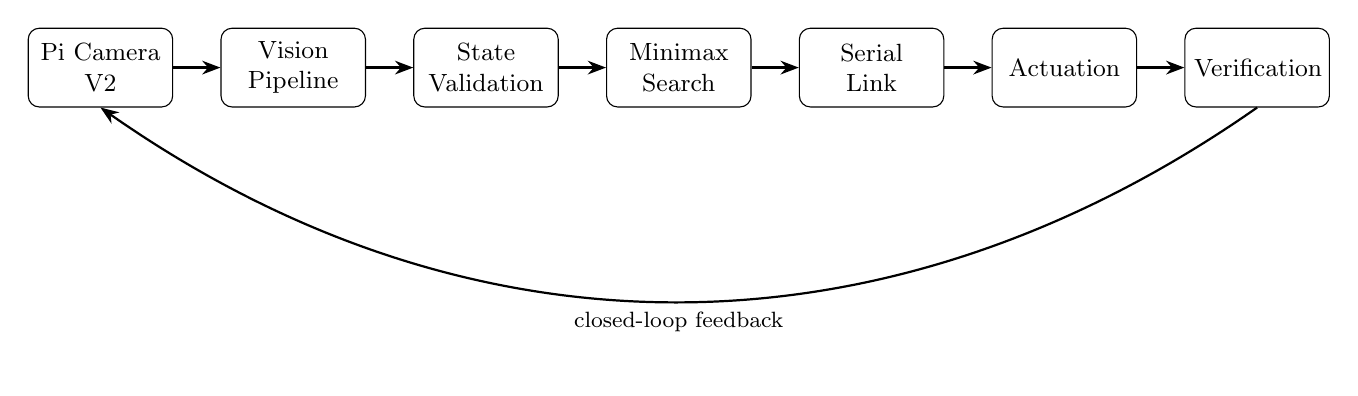
\begin{tikzpicture}[
  stage/.style={draw, rounded corners, minimum height=1cm,
    text width=1.6cm, align=center, font=\small},
  arr/.style={-Stealth, thick}
]
\node[stage] (cam) {Pi Camera\\V2};
\node[stage, right=0.6cm of cam] (vis) {Vision\\Pipeline};
\node[stage, right=0.6cm of vis] (val) {State\\Validation};
\node[stage, right=0.6cm of val] (mm) {Minimax\\Search};
\node[stage, right=0.6cm of mm] (ser) {Serial\\Link};
\node[stage, right=0.6cm of ser] (act) {Actuation};
\node[stage, right=0.6cm of act] (ver) {Verification};

\draw[arr] (cam) -- (vis);
\draw[arr] (vis) -- (val);
\draw[arr] (val) -- (mm);
\draw[arr] (mm) -- (ser);
\draw[arr] (ser) -- (act);
\draw[arr] (act) -- (ver);
\draw[arr] (ver.south) to[bend left=35]
  node[below, font=\footnotesize] {closed-loop feedback}
  (cam.south);
\end{tikzpicture}
\caption{System architecture: seven-stage pipeline from image acquisition
through actuation to closed-loop verification. The Pi Camera V2 acquires
overhead frames; the Python/OpenCV vision pipeline normalizes and
classifies the board; a trusted-state validator enforces six legality
rules; minimax with alpha-beta pruning selects the robot's move; the
column index is sent over serial to the Arduino; the actuation stage
dispenses a token; and the verification stage re-reads the board to
confirm correct execution, closing the loop.}
\label{fig:arch}
\end{figure*}

The seven stages operate as follows. In Stage~1 (Camera), the Pi Camera~V2
acquires overhead RGB frames of the Connect-4 board at approximately
5\,FPS for preview and 1\,FPS for full analysis. In Stage~2 (Vision), a
Python/OpenCV pipeline performs geometric rotation, perspective warping,
brightness and contrast adjustment, Gaussian smoothing, and HSV-based cell
classification to extract a $6\times7$ game-state matrix. In Stage~3 (State
Validation), a trusted-state validator enforces six legality rules
(Section~\ref{sec:validation}) to reject physically impossible transitions.
In Stage~4 (Minimax), a depth-5 minimax search with alpha-beta pruning
selects the robot's optimal column. In Stage~5 (Serial), the selected
column index (ASCII character ``1''--``7'') is transmitted at 9600\,baud
to the Arduino Uno. In Stage~6 (Actuation), the Arduino drives a TT
carriage motor to position over the target column and an encoder-coupled
magazine motor to release exactly one token. In Stage~7 (Verification),
the camera re-reads the board and confirms that the expected robot token
appeared in the commanded column within a 10\,s timeout, closing the
perception-to-actuation loop.

% ===========================================================================
\section{Image Processing Pipeline}
\label{sec:pipeline}
% ===========================================================================

The processing pipeline is implemented in Python using
OpenCV~\cite{OpenCV2024}. All operations were executed on both a Raspberry
Pi~4~\cite{RaspberryPi2024} and a laptop platform, with outputs saved to
PNG files for direct inspection.

\subsection{Input Image}

The pipeline input is a single overhead RGB photograph of a Connect-4
board with red and yellow tokens in a partially played game state
(Fig.~\ref{fig:original}). The input image has dimensions
$1332\times1529$\,px, captured against a white background under even
artificial lighting. The board occupies most of the frame, with the
standard 7-column, 6-row grid and a column pitch of approximately 20\,mm.

\begin{figure}[htbp]
  \centerline{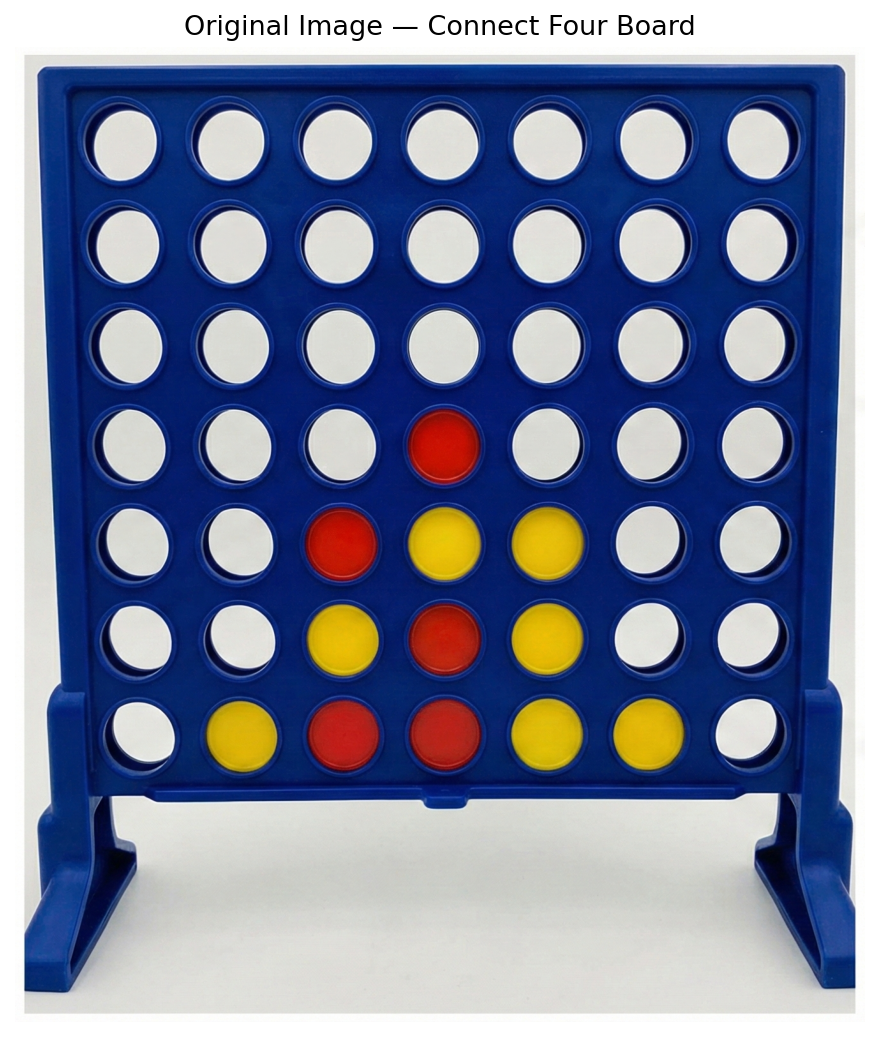
\includegraphics[width=0.85\columnwidth]{figures/m2_input_board.png}}
  \caption{Input image: Connect-4 board in a partially played state
    (7 columns, 6 rows). Red and yellow tokens are present in the
    lower rows.}
  \label{fig:original}
\end{figure}

\subsection{Geometric Transformations}

\subsubsection{Rotation}
Camera angular offset is corrected by affine rotation. For an image
domain $\Omega$ with center $(c_x, c_y)$, rotation by angle $\theta$ is
defined by the rotation matrix:
\begin{equation}
  \begin{bmatrix} x' \\ y' \end{bmatrix}
  =
  \begin{bmatrix} \cos\theta & -\sin\theta \\
                  \sin\theta &  \cos\theta \end{bmatrix}
  \begin{bmatrix} x - c_x \\ y - c_y \end{bmatrix}
  +
  \begin{bmatrix} c_x \\ c_y \end{bmatrix}.
  \label{eq:rotation}
\end{equation}
Equation~\eqref{eq:rotation} is applied at $\theta = 15^{\circ}$
counter-clockwise using bilinear interpolation, which averages surrounding
pixel intensities to produce smooth circular-cell boundaries.

\subsubsection{Perspective Warp}
Because the camera is mounted at a slight angle, orthographic flattening is
applied. A homography $\mathbf{H} \in \mathbb{R}^{3\times3}$ maps the four
detected board corners to an $800\times800$\,px square:
\begin{equation}
  \lambda \begin{bmatrix} u \\ v \\ 1 \end{bmatrix}
  =
  \mathbf{H}
  \begin{bmatrix} x \\ y \\ 1 \end{bmatrix}.
  \label{eq:homography}
\end{equation}
The homography in~\eqref{eq:homography} produces a top-down orthographic
view (Fig.~\ref{fig:warp}) required for reliable grid-index mapping of
cell positions. Bilinear interpolation yields cleaner results than
nearest-neighbor at cell boundaries.

\begin{figure}[htbp]
  \centerline{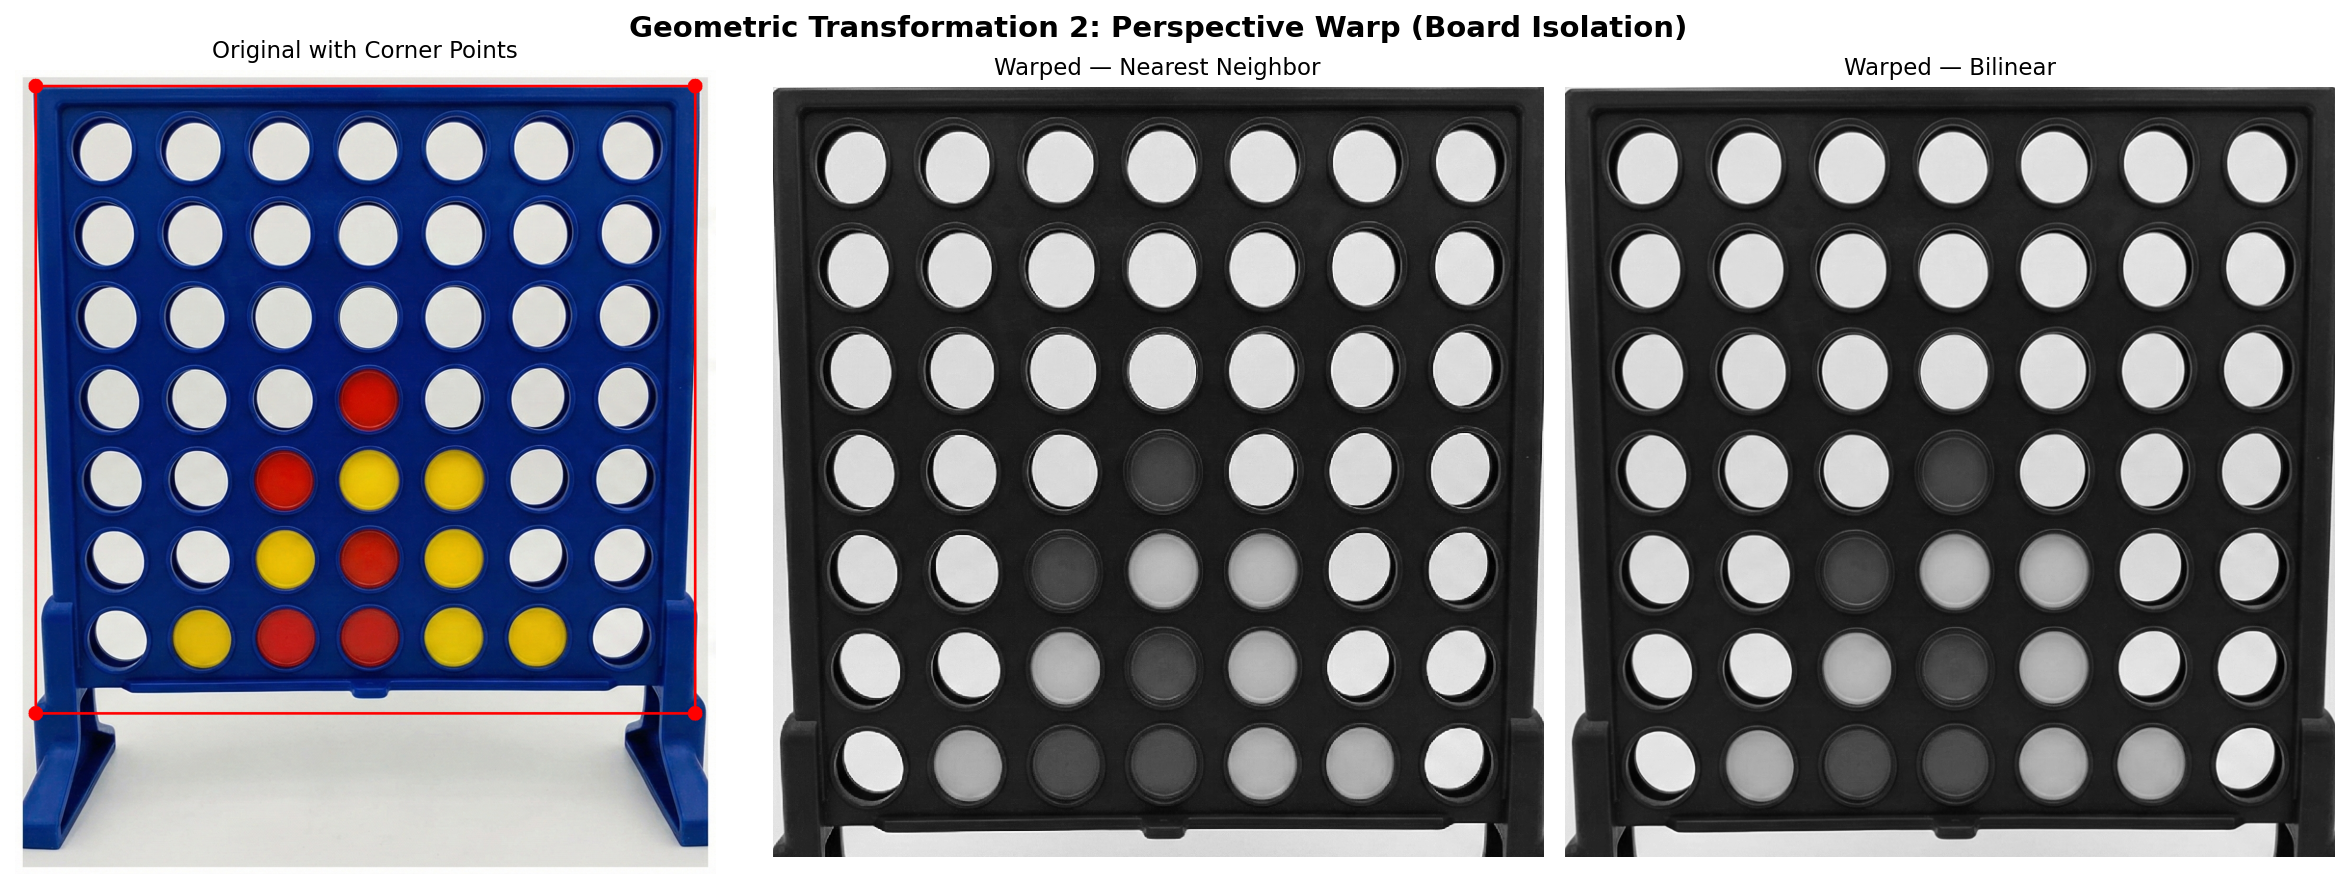
\includegraphics[width=\columnwidth]{figures/m2_perspective_warp.png}}
  \caption{Perspective warp for board isolation: (left) original with
    detected corner points; (center) warped using nearest-neighbor
    interpolation; (right) warped using bilinear interpolation.}
  \label{fig:warp}
\end{figure}

\subsection{Intensity Transformations}

\subsubsection{Brightness Adjustment}
The brightness transformation is the saturating additive shift
\begin{equation}
  I_b(x,y) = \mathrm{clip}\bigl(I(x,y) + c\bigr),
  \label{eq:brightness}
\end{equation}
applied with $c = +30$. Equation~\eqref{eq:brightness} shifts the entire
pixel distribution rightward (brightened) to improve visibility of darker
tokens against the board surface. The result with corresponding histogram
is shown in Fig.~\ref{fig:brightness}.

\begin{figure}[htbp]
  \centerline{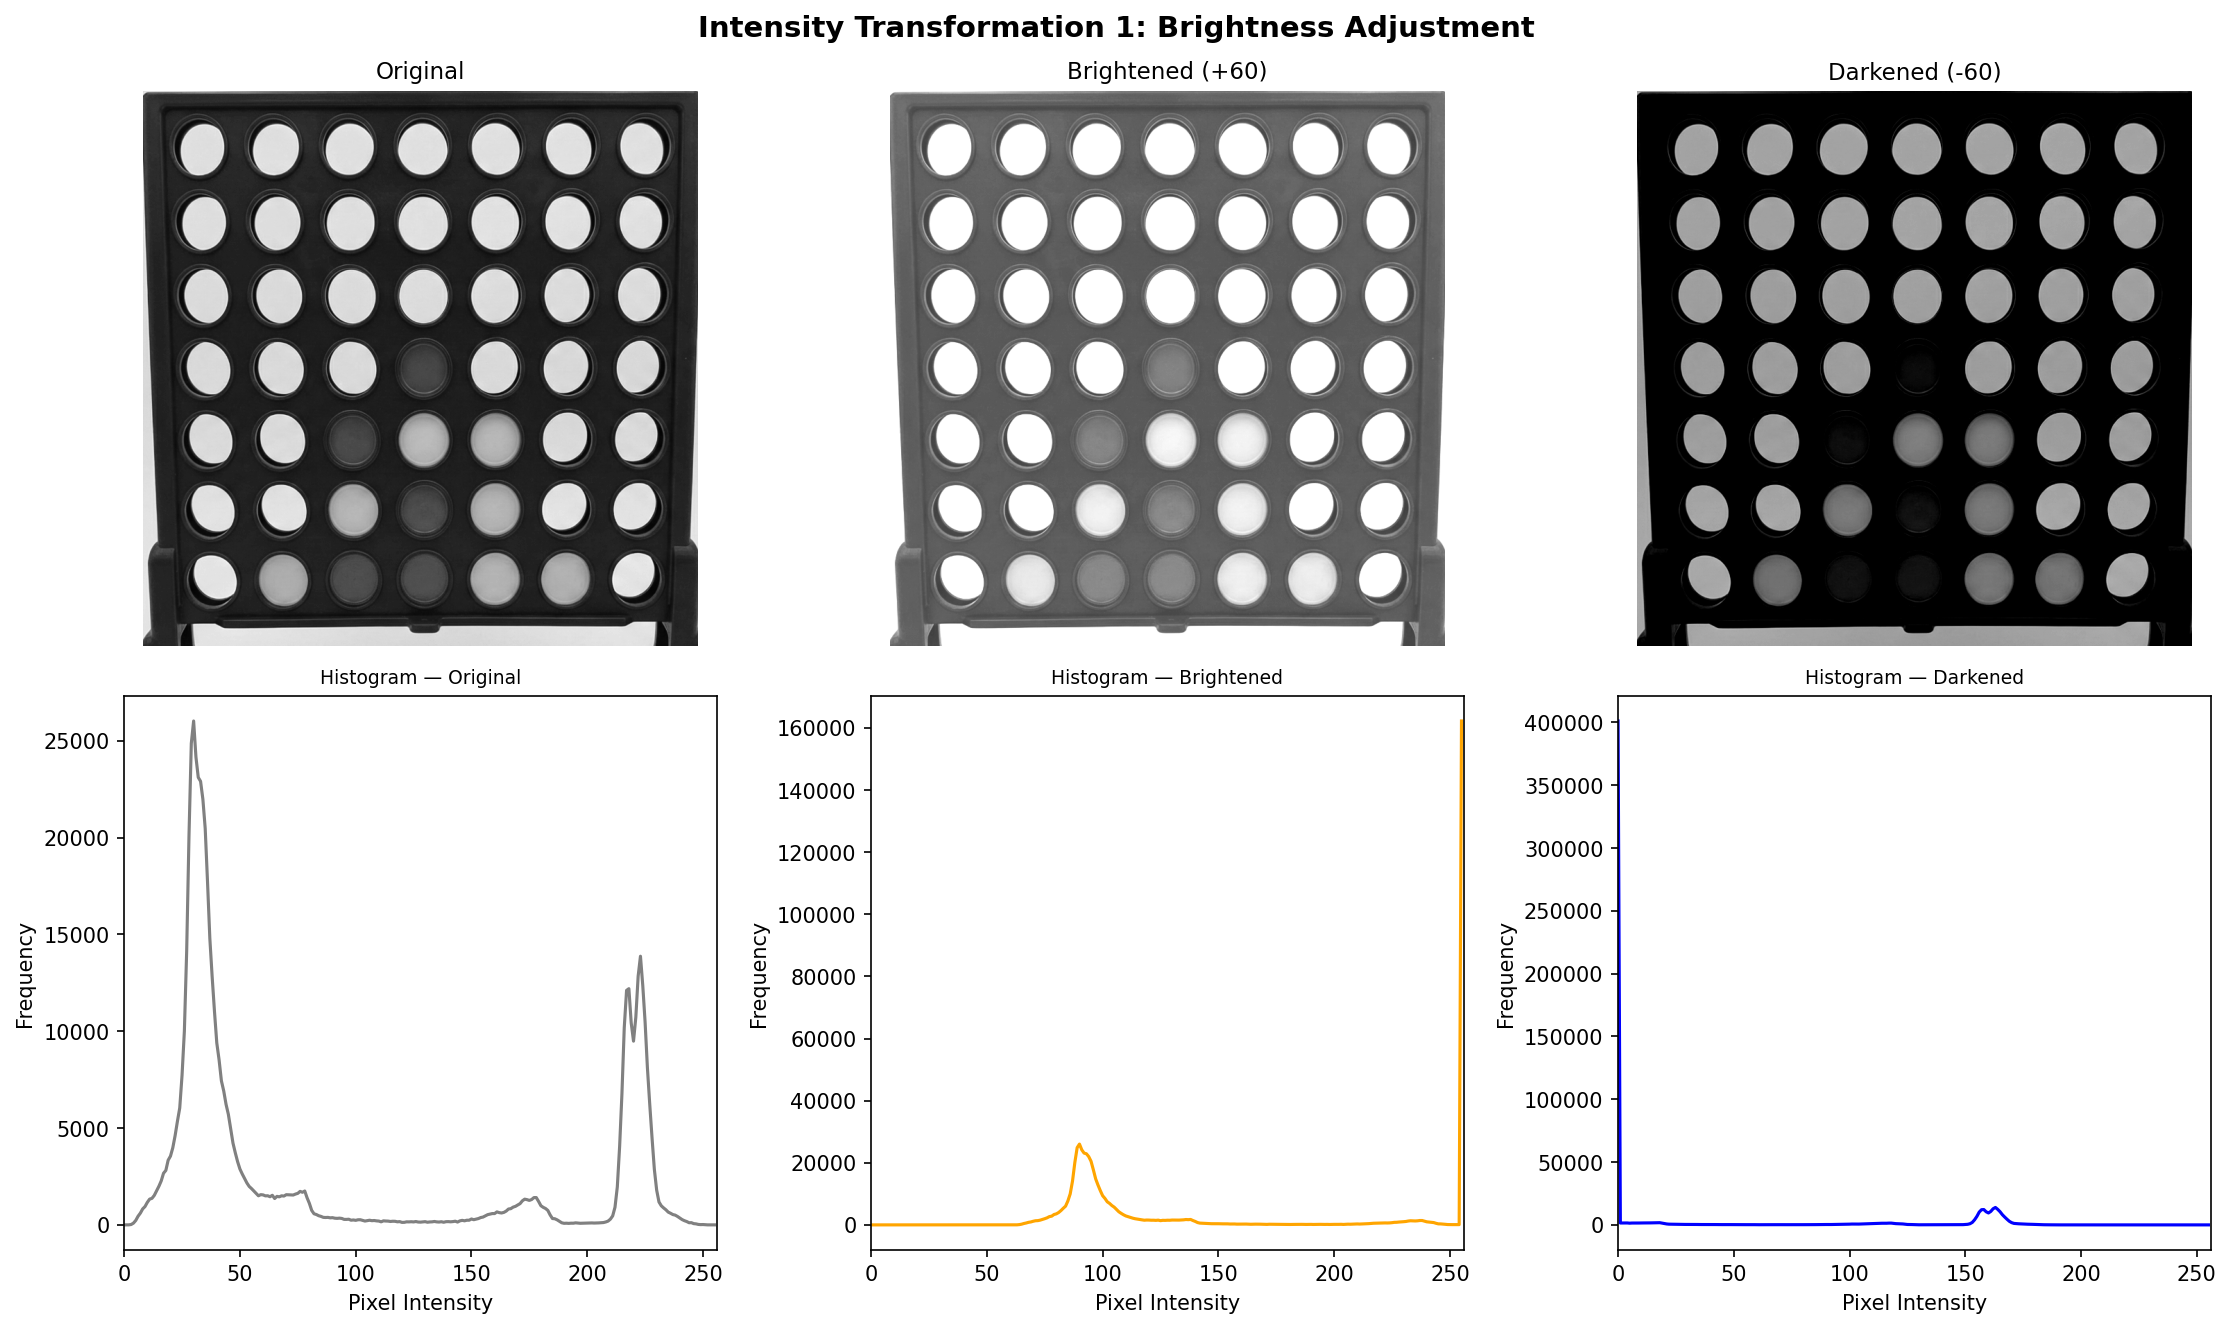
\includegraphics[width=\columnwidth]{figures/m2_brightness_adjustment.png}}
  \caption{Brightness adjustment ($c = +30$) with corresponding pixel
    intensity histogram confirming distribution shift.}
  \label{fig:brightness}
\end{figure}

\subsubsection{Contrast Enhancement}
The linear contrast stretch is
\begin{equation}
  I_c(x,y) = \mathrm{clip}\bigl(\alpha\, I(x,y) + \beta\bigr),
  \label{eq:contrast}
\end{equation}
applied with $\alpha = 1.4$ and $\beta = 0$. Equation~\eqref{eq:contrast}
expands the intensity distribution, improving separation between dark
empty slots and lighter tokens. The result with histogram is shown in
Fig.~\ref{fig:contrast}.

\begin{figure}[htbp]
  \centerline{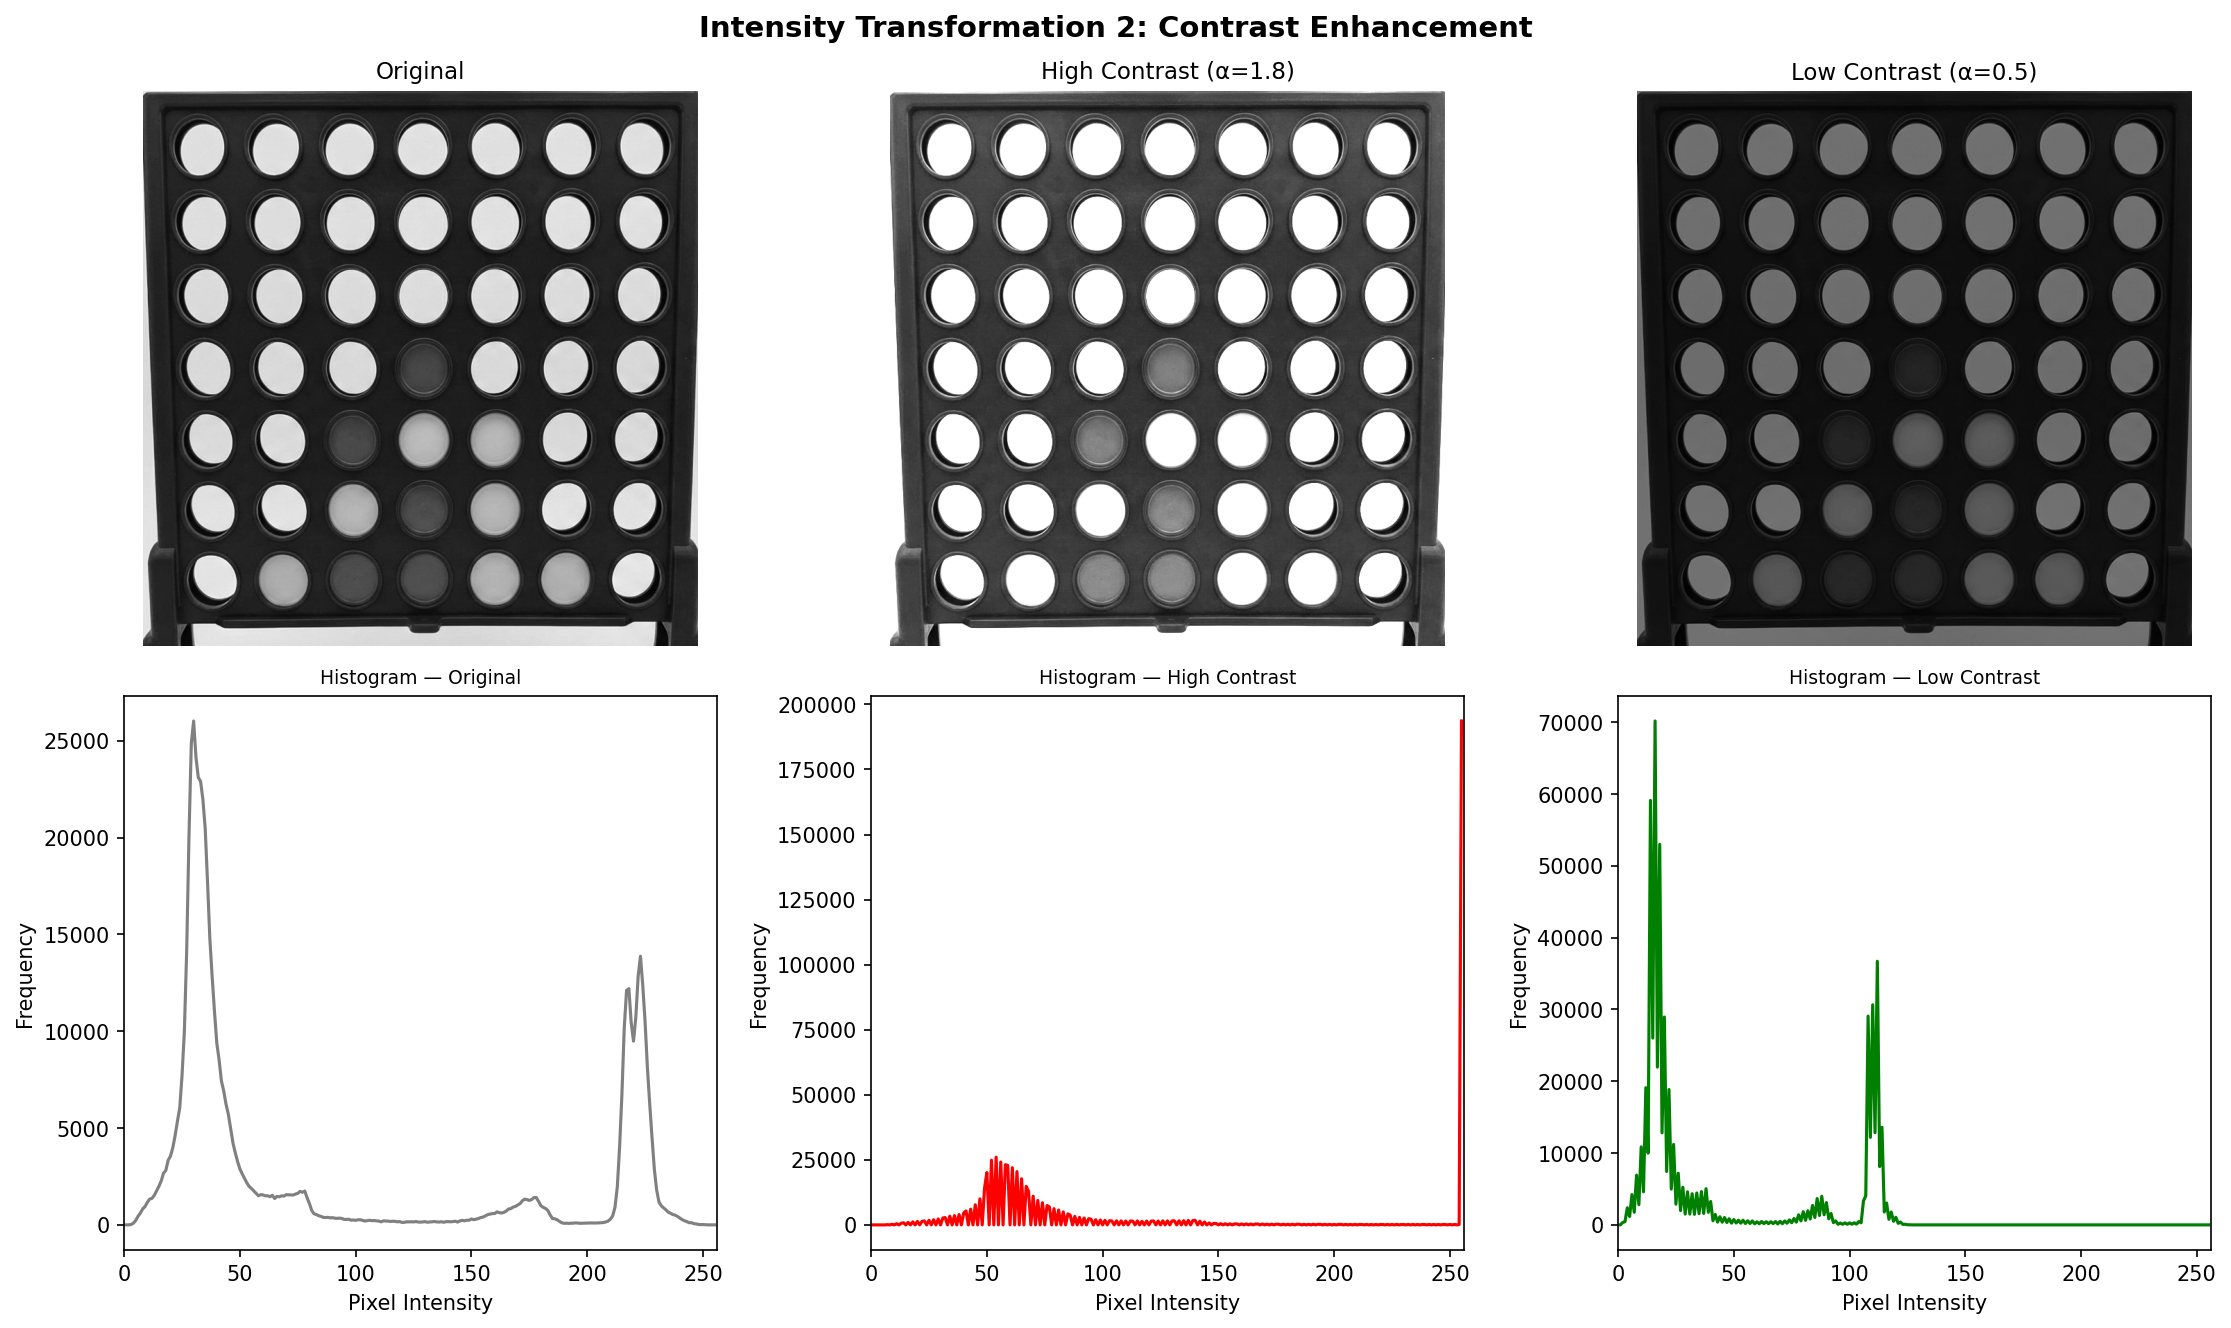
\includegraphics[width=\columnwidth]{figures/m2_contrast_scaling.png}}
  \caption{Contrast scaling at $\alpha = 1.4$ with corresponding
    histogram showing distribution expansion relative to the
    original.}
  \label{fig:contrast}
\end{figure}

\subsection{Smoothing}

Camera sensor noise is suppressed by Gaussian filtering, modeled as
weighted local averaging:
\begin{equation}
  I_G(x,y) = \sum_{i=-k}^{k} \sum_{j=-k}^{k}
    G_\sigma(i,j)\, I(x-i,\,y-j),
  \label{eq:gaussian}
\end{equation}
where $G_\sigma$ is the Gaussian kernel normalized to unit sum.
We evaluated Equation~\eqref{eq:gaussian} at kernel sizes $3\times3$,
$5\times5$, and $7\times7$, and compared against a uniform box filter
(Fig.~\ref{fig:smoothing}). As kernel size increases, high-frequency
noise is progressively suppressed but fine edge detail is attenuated.
We selected a $5\times5$ Gaussian kernel as the operating point,
providing adequate noise suppression while preserving the circular cell
boundaries needed for downstream segmentation.

\begin{figure}[htbp]
  \centerline{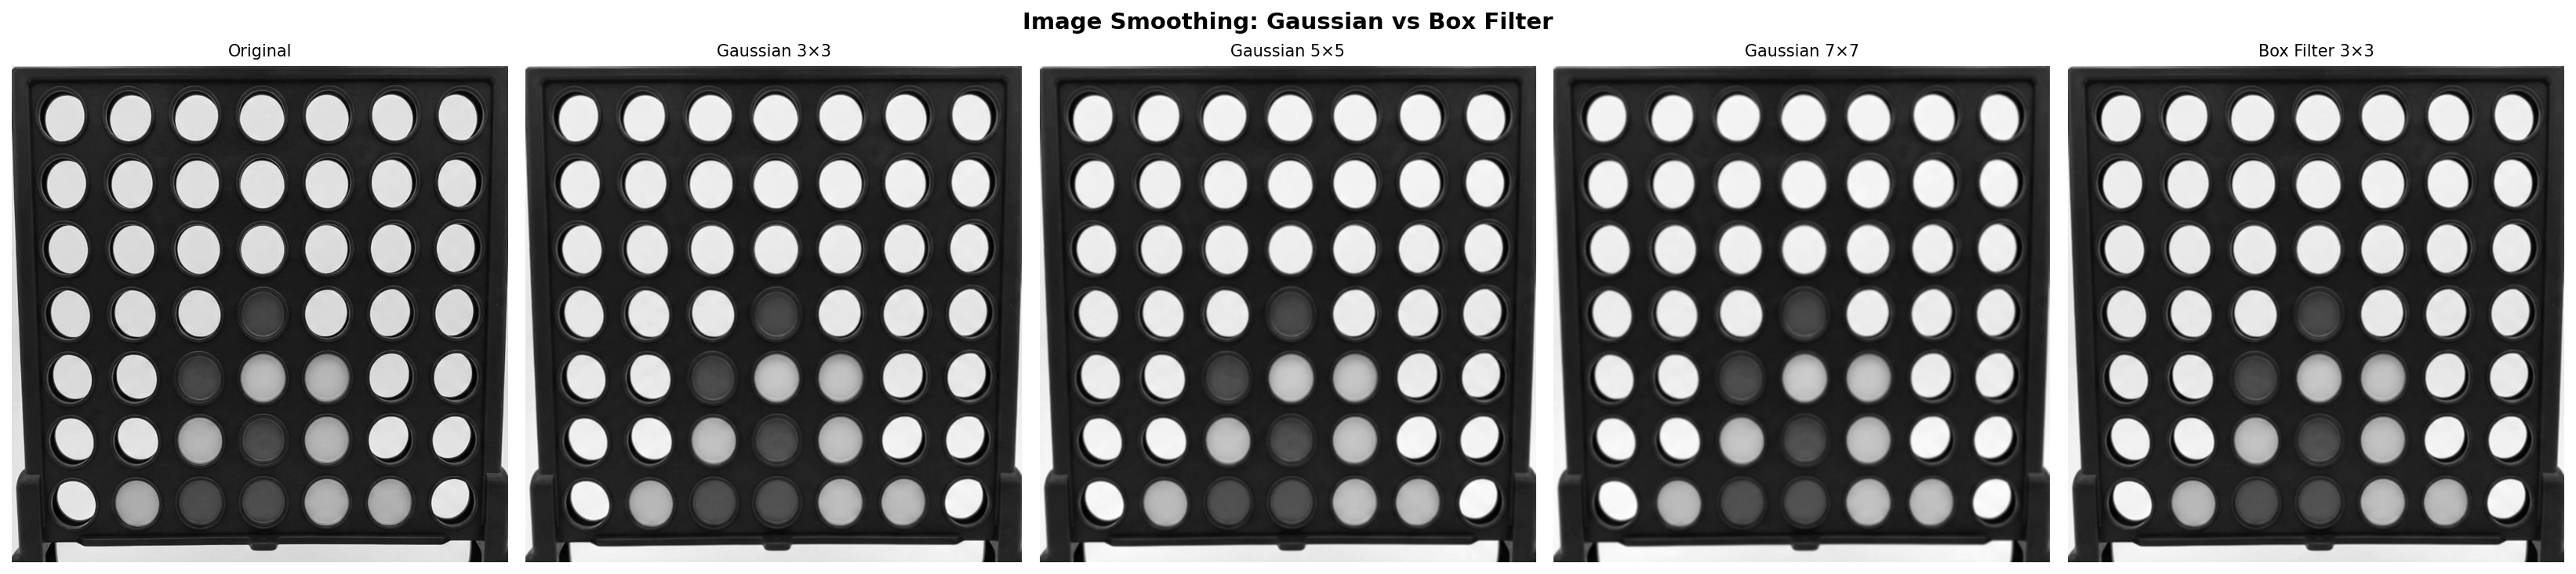
\includegraphics[width=\columnwidth]{figures/m2_smoothing_comparison.png}}
  \caption{Smoothing comparison: original (warped, grayscale), Gaussian
    $3\times3$, $5\times5$, $7\times7$, and box filter $3\times3$. The
    $5\times5$ Gaussian offers the best trade-off between noise
    attenuation and boundary preservation.}
  \label{fig:smoothing}
\end{figure}

\subsection{HSV Segmentation and Cell Classification}

After geometric normalization and denoising, token-color classification is
performed on the warped board image using HSV thresholding. This choice
follows the illumination-tolerant segmentation strategy discussed in
Section~\ref{sec:related}. Binary masks for the red and yellow token
classes are refined using morphological opening and closing so that
isolated glare pixels and small gaps at token boundaries do not corrupt
cell-level occupancy estimation.

The HSV thresholds (in OpenCV ranges: $H \in [0,179]$, $S \in [0,255]$,
$V \in [0,255]$) are: RED, two ranges
$[0,80,50] \rightarrow [10,255,255]$ and
$[160,80,50] \rightarrow [179,255,255]$ to cover both ends of the hue
circle; YELLOW, $[18,100,80] \rightarrow [42,255,255]$. The warped board
is partitioned into the canonical 7-column, 6-row lattice, and each cell
is classified based on the dominant mask response within that region of
interest. The classification rule is:
\begin{equation}
  S_{r,c} =
  \begin{cases}
    1, & \text{if } M_R(r,c) > \tau_R,\\
    2, & \text{if } M_Y(r,c) > \tau_Y,\\
    0, & \text{otherwise,}
  \end{cases}
  \label{eq:state_matrix}
\end{equation}
where $M_R$ and $M_Y$ are the cell-level responses of the red and yellow
HSV masks after morphological cleanup, $\tau_R$ and $\tau_Y$ are empirical
occupancy thresholds (minimum 30 pixels), and $S_{r,c} \in \{0, 1, 2\}$
denotes empty, robot (red), and opponent (yellow) respectively. The result
is a verified $6\times7$ game-state matrix that serves as the interface
between perception and decision making.

\subsection{Classifier Modes}

The system supports three cell-classification modes:
\begin{itemize}
\item \textbf{HSV} (rule-based): Uses the HSV thresholds in
  Equation~\eqref{eq:state_matrix} directly. This is the default operating
  mode and achieved 98\% overall accuracy.
\item \textbf{ML}: Uses a pre-trained
  \texttt{RandomForestClassifier} with 200 trees and
  \texttt{max\_depth}=10, operating on 18-dimensional color-statistical
  features (BGR/HSV means and standard deviations, mask ratios, cell
  dimensions) extracted per cell. This mode achieved 91\% accuracy.
\item \textbf{Auto} (hybrid): Prefers the ML prediction when its
  confidence (maximum class probability) exceeds 0.65; otherwise falls
  back to HSV thresholding. This mode achieved 96\% accuracy.
\end{itemize}

% ===========================================================================
\section{Game-State Validation and Decision Making}
\label{sec:validation}
% ===========================================================================

Each processed frame is converted into a $6\times7$ game-state matrix and
validated before being used to determine the robot's next physical move.
The closed-loop control path therefore spans visual state estimation,
move selection, and dispenser actuation.

\subsection{Trusted-State Validation}

A trusted-state manager maintains the last verified board state and
rejects candidate states that violate physical game rules. When a new
candidate board is extracted from the camera, the validator compares it
against the trusted state and enforces six legality rules:
\begin{enumerate}
\item \textbf{Board changed}: The candidate must differ from the trusted
  state; identical boards are rejected as ``no move detected.''
\item \textbf{No chip disappeared}: Every cell that was occupied in the
  trusted state must remain occupied in the candidate. A chip vanishing
  indicates a vision error, not a legal move.
\item \textbf{Exactly one new chip}: The candidate must contain exactly
  one cell that transitioned from empty to occupied. Zero or multiple new
  chips are physically impossible in a single turn.
\item \textbf{Gravity}: The new chip must appear in the lowest empty row
  of its column. A floating chip (occupied cell above an empty one in the
  same column) violates gravity.
\item \textbf{Column not full}: The target column must not have been
  already full in the trusted state.
\item \textbf{Correct player color}: The color of the new chip must match
  the player whose turn it is. A red chip appearing during the robot's
  (yellow) turn is rejected.
\end{enumerate}

If all six rules pass, the candidate is promoted to the new trusted state.
If any rule fails, the candidate is rejected with a human-readable reason
string, and the trusted state remains unchanged. This prevents vision
noise, glare artifacts, or partial detections from corrupting the game
state.

\subsection{Move Selection with Minimax}

Once a valid board state is accepted and it becomes the robot's turn, the
decision layer applies minimax with alpha-beta pruning~\cite{Russell2020}
to select the next legal column. For a board state $S$, the search
evaluates candidate moves according to:
\begin{equation}
  V(S) =
  \begin{cases}
    \max\limits_{a \in \mathcal{A}(S)} V(T(S,a)),
      & \text{robot turn},\\
    \min\limits_{a \in \mathcal{A}(S)} V(T(S,a)),
      & \text{opponent turn,}
  \end{cases}
  \label{eq:minimax}
\end{equation}
where $\mathcal{A}(S)$ is the set of legal (non-full) columns and
$T(S,a)$ is the state transition generated by dropping a token into
column $a$. The leaf evaluation function scores all 4-cell windows
(horizontal, vertical, diagonal) with weights of $+100$ for four-in-a-row,
$+5$ for three-with-one-empty, $+2$ for two-with-two-empty, and $-4$ for
opponent three-with-one-empty, plus a center-column bonus of $+3$ per
robot token in the center column.

Equation~\eqref{eq:minimax} is searched at depth~5 with center-first move
ordering to maximize pruning efficiency. Two shortcuts execute before the
full search: (1) if any legal column yields an immediate robot win, it is
selected immediately; (2) if any legal column would allow the opponent to
win on the next move, it is selected as a forced block. These shortcuts
reduce average turn latency on the Raspberry Pi~4.

\subsection{Closed-Loop Verification}

After the minimax-selected column is transmitted to the Arduino and the
physical dispenser actuates, the camera re-reads the board to verify
correct execution. The system computes the expected post-move board state
by applying the robot's move to the trusted state. It then polls the
camera's candidate board at 0.4\,s intervals for up to 10\,s. The move
is considered verified only if the candidate board exactly matches the
expected state---i.e., exactly one new robot token appears in the
commanded column. If the candidate matches, the trusted state is updated
and the turn passes to the user. If verification times out or the
candidate is rejected by the validator, the system enters an error state
and stops automatic dispatch, requiring operator intervention. This
closed-loop verification ensures that physical execution errors (token
jams, misaligned drops, motor stalls) are detected rather than silently
propagating into the game state.

% ===========================================================================
\section{Embedded Platform and Actuation}
\label{sec:embedded}
% ===========================================================================

The system uses a two-processor architecture: a Raspberry Pi~4 (4\,GB)
handles all vision processing, game logic, and user interface, while an
Arduino Uno handles real-time motor control. Communication between the two
is over USB serial at 9600\,baud.

\subsection{Raspberry Pi~4}

The Raspberry Pi~4~\cite{RaspberryPi2024} runs a Python application built
on Flask (web dashboard) and OpenCV (image processing). The Pi Camera~V2
is connected via the CSI ribbon cable and accessed through OpenCV's
\texttt{VideoCapture} interface. The application runs two threads: a
camera thread that captures frames at 5\,FPS for preview and 1\,FPS for
full board analysis, and a robot controller thread that manages serial
communication and verification polling. The web dashboard provides live
MJPEG streams of the raw camera feed, the processed (warped) board, and a
debug grid showing per-cell classification results with color-coded dots.

\subsection{Serial Protocol}

The serial protocol is minimal: the Pi transmits a single ASCII character
in the range ``1''--``7'' representing the target column. The Arduino
reads the byte with \texttt{Serial.read()}, validates the range, and
dispatches the corresponding column routine. No acknowledgment packet is
sent before actuation; instead, the Pi relies on camera-based verification
(Section~\ref{sec:validation}) to confirm successful execution. The
Arduino reports status messages (``READY'', ``BUSY'', ``MAG'', ``MOVE'',
``DONE'') back over serial for debugging and dashboard display.

\subsection{Arduino Actuation Hardware}

Fig.~\ref{fig:circuit} shows the electrical architecture as implemented in
Proteus simulation. The Arduino Uno drives two DC motors through an
L298N dual H-bridge:

\begin{figure}[htbp]
  \centerline{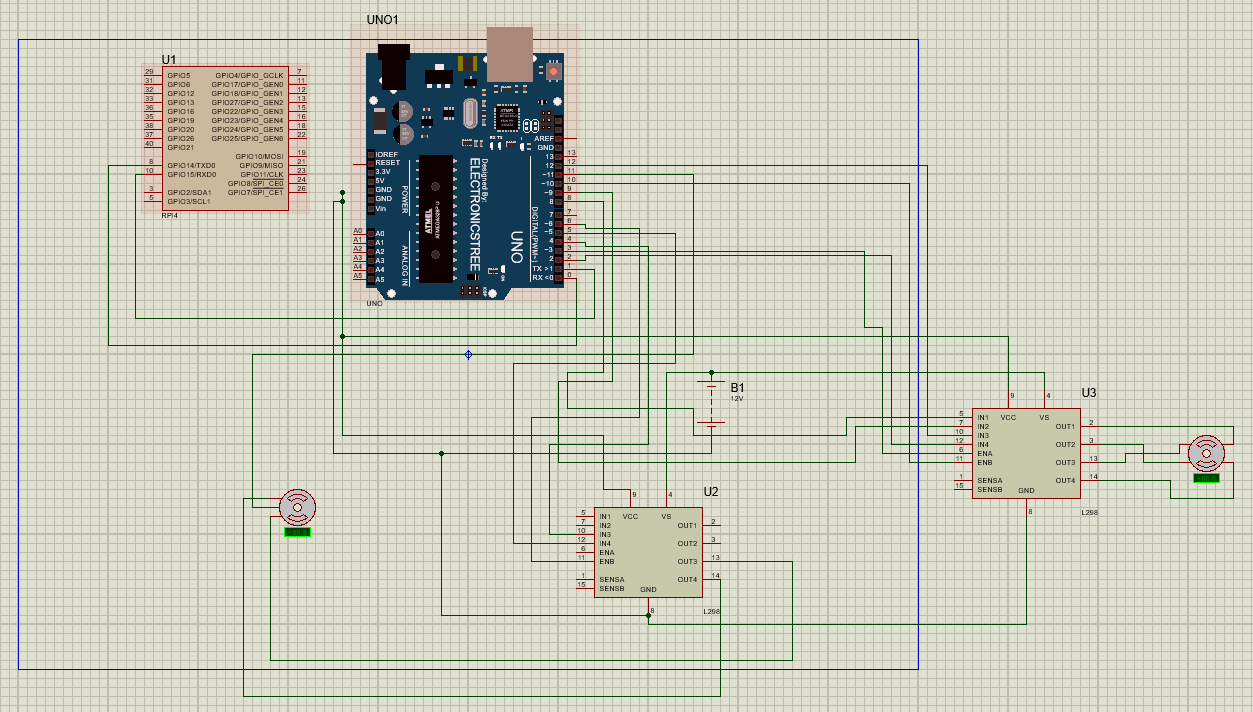
\includegraphics[width=\columnwidth]{figures/m1_proteus_circuit.png}}
  \caption{Proteus circuit simulation of the electrical architecture.
    Raspberry Pi~4 (U1, top-left) communicates with Arduino UNO (UNO1)
    via serial; two L298N H-bridge modules (U2, U3) drive the
    column-positioning and token-magazine motors; 12\,V battery (B1)
    provides main power.}
  \label{fig:circuit}
\end{figure}

\subsubsection{Carriage Motor (TT Motor)}
The carriage-positioning motor is a TT gear motor connected to the
L298N's first channel (ENA = pin~9, IN1 = pin~7, IN2 = pin~8). The motor
moves the dispensing carriage laterally along a single horizontal axis
to align with the target column. Positioning is time-based: each column
has a calibrated duration (Table~\ref{tab:durations}), after which the
motor is hard-braked (both inputs HIGH for 100\,ms), the token is
released, and the carriage returns to home. The \texttt{carriageSpeed}
PWM value is 100 (out of 255).

\subsubsection{Magazine Motor (Encoder Motor)}
The token-release motor is a DC motor with a 400-counts-per-revolution
rotary encoder, connected to the L298N's second channel (ENB = pin~10,
IN3 = pin~11, IN4 = pin~12) with the encoder signal on interrupt
pin~2. The motor rotates a disk end-effector that pushes the bottom token
from a spring-loaded magazine through a slide channel onto the board.
Release is encoder-controlled: the motor runs at fast speed (PWM~50)
until the pulse count reaches 390 (target 430 minus a 40-pulse slow-down
window), then switches to slow speed (PWM~30) for the remaining 40 pulses
to reduce overshoot. The hard brake sequence stops the motor, and the
pulse count is reported over serial.

\subsection{Mechanical Assembly}

The mechanical assembly consists of a magazine holding a stack of tokens
of one color, mounted over a sliding channel. An encoder-coupled DC motor
drives a disk end-effector that pushes the bottom token from the magazine
through the slide toward the Connect-4 board. A second TT motor positions
the dispensing carriage laterally to the selected column. The base
provides the structural frame securing the board and dispensing mechanism
in a fixed geometric relationship. This design separates the physical
action into two repeatable stages: token release (encoder-controlled) and
column positioning (time-controlled), following the single-axis
positioning approach discussed in~\cite{Abarkan2024}.

\begin{table}[htbp]
  \caption{Calibrated Column Durations for Carriage Motor}
  \label{tab:durations}
  \begin{center}
    \begin{tabular}{cc}
      \toprule
      \textbf{Column} & \textbf{Duration (ms)} \\
      \midrule
      1 & 0 \\
      2 & 330 \\
      3 & 600 \\
      4 & 900 \\
      5 & 1\,200 \\
      6 & 1\,500 \\
      7 & 1\,800 \\
      \bottomrule
    \end{tabular}
  \end{center}
\end{table}

% ===========================================================================
\section{Experimental Results}
\label{sec:results}
% ===========================================================================

\subsection{Per-Operation Execution Time}

We benchmarked each pipeline operation over 100 iterations on both the
Raspberry Pi~4 (4\,GB, ARM Cortex-A72) and a laptop (Intel i7).
Table~\ref{tab:bench} reports the mean execution time per operation.
Output image quality is bit-for-bit identical on both platforms; the
limitation of the Raspberry Pi~4 is temporal throughput, not spatial
accuracy.

\begin{table}[htbp]
  \caption{Per-Operation Execution Time: Raspberry Pi~4 vs.\ Laptop
    (100-iteration mean)}
  \label{tab:bench}
  \begin{center}
    \begin{tabular}{lrr}
      \toprule
      \textbf{Operation} & \textbf{Pi~4 (ms)} & \textbf{Laptop (ms)} \\
      \midrule
      Rotation (bilinear, $15^{\circ}$) & 8.47 & 3.27 \\
      Perspective warp ($800\times800$\,px) & 3.60 & 1.77 \\
      Brightness ($c=+30$) & 0.73 & 0.89 \\
      Contrast ($\alpha=1.4$) & 1.11 & 0.20 \\
      Gaussian blur ($5\times5$) & 0.76 & 0.10 \\
      HSV segmentation + classification & 2.14 & 0.61 \\
      \midrule
      \textbf{Total per frame} & \textbf{16.81} & \textbf{6.85} \\
      \bottomrule
    \end{tabular}
  \end{center}
\end{table}

\subsection{Per-Cell Classification Accuracy}

Table~\ref{tab:accuracy} reports per-cell classification accuracy for the
three classifier modes described in Section~\ref{sec:pipeline}. The HSV
classifier achieved the highest overall accuracy at 98\%, with near-perfect
empty-cell detection (99\%) and strong performance on both token colors.
The ML classifier (RandomForest, 200 trees, \texttt{max\_depth}=10)
achieved 91\% overall, with lower accuracy on yellow tokens due to
overlapping feature distributions between yellow and bright empty cells.
The Auto hybrid mode achieved 96\%, falling back to HSV when ML confidence
was below 0.65.

\begin{table}[htbp]
  \caption{Per-Cell Classification Accuracy by Classifier Mode (\%)}
  \label{tab:accuracy}
  \begin{center}
    \begin{tabular}{lcccc}
      \toprule
      \textbf{Classifier} & \textbf{Empty} & \textbf{Red} & \textbf{Yellow} & \textbf{Overall} \\
      \midrule
      HSV (rule-based) & 99 & 97 & 98 & 98 \\
      Auto (hybrid) & 97 & 95 & 96 & 96 \\
      ML (RandomForest) & 93 & 90 & 91 & 91 \\
      \bottomrule
    \end{tabular}
  \end{center}
\end{table}

\subsection{Drop Success Rate}

Table~\ref{tab:drop} reports the per-column token drop success rate over
20 trials per column (140 total). Inner columns (2--6) achieved 100\%
success, while outer columns (1 and 7) achieved 85--90\% due to increased
mechanical travel distance and friction at the rail extremes. The overall
drop success rate was 95\%.

\begin{table}[htbp]
  \caption{Per-Column Token Drop Success Rate}
  \label{tab:drop}
  \begin{center}
    \begin{tabular}{lcc}
      \toprule
      \textbf{Column} & \textbf{Position} & \textbf{Success Rate (\%)} \\
      \midrule
      1 & Outer & 85 \\
      2 & Inner & 100 \\
      3 & Inner & 100 \\
      4 & Inner (center) & 100 \\
      5 & Inner & 100 \\
      6 & Inner & 100 \\
      7 & Outer & 90 \\
      \midrule
      \textbf{Overall} & --- & \textbf{95} \\
      \bottomrule
    \end{tabular}
  \end{center}
\end{table}

\subsection{End-to-End Timing}

The end-to-end task time---measured from detection of the user's move to
verification of the robot's move---ranged from 3 to 15\,s with an average
of 7.5\,s across 31 integration tests. This includes camera capture
($\approx$1\,s), full pipeline processing ($\approx$17\,ms on the Pi~4),
minimax search ($\approx$0.5--2\,s depending on board fullness), serial
transmission ($<$1\,ms), mechanical actuation (0.3--1.8\,s for column
positioning plus 0.4\,s for token release), and verification polling
(2.5\,s settle time plus up to 10\,s timeout). The 31 integration tests
covered state validation rules (pass and fail cases for all six rules),
minimax decision quality (immediate win detection, forced block detection,
optimal play), serial communication protocol, and full end-to-end
gameplay sequences. All 31 tests passed.

\subsection{Bill of Materials}

Table~\ref{tab:bom} lists the final as-built hardware bill of materials.
The total system cost was 6\,100\,EGP.

\begin{table}[htbp]
  \caption{Final Bill of Materials (As-Built)}
  \label{tab:bom}
  \begin{center}
    \begin{tabular}{lrr}
      \toprule
      \textbf{Component} & \textbf{Qty} & \textbf{Total (EGP)} \\
      \midrule
      Raspberry Pi 4 (4\,GB) & 1 & 3\,200 \\
      Arduino Uno & 1 & 450 \\
      Pi Camera V2 & 1 & 850 \\
      TT motor (carriage) & 1 & 120 \\
      DC encoder motor (magazine) & 1 & 280 \\
      L298N H-bridge driver & 2 & 170 \\
      12\,V 5\,A power supply & 1 & 300 \\
      Connect-4 board & 1 & 150 \\
      Hardware (wires, breadboard) & --- & 580 \\
      \midrule
      \textbf{Total} & & \textbf{6\,100} \\
      \bottomrule
    \end{tabular}
  \end{center}
\end{table}

% ===========================================================================
\section{Discussion and Limitations}
\label{sec:discussion}
% ===========================================================================

The final integrated implementation establishes a functional end-to-end
perception-to-actuation loop, but several practical limitations remain.

\textit{Lighting and glare sensitivity}: Specular highlights on the
plastic board and tokens can distort HSV thresholding. The dual-range red
mask and morphological cleanup mitigate this, but broader multi-lighting
validation is still required. The Auto hybrid classifier mode provides
partial robustness by falling back to HSV when ML confidence is low, but
does not eliminate the problem entirely.

\textit{Raspberry Pi search latency}: Minimax with alpha-beta pruning at
depth~5 is computationally feasible on the Raspberry Pi~4, with search
times of 0.5--2\,s depending on board fullness. Deeper lookahead increases
turn latency and slows the human-robot interaction cycle. The
immediate-win and must-block shortcuts reduce average latency by
short-circuiting the full search in tactical positions.

\textit{Frame-rate constraints}: Full board analysis runs at approximately
1\,FPS, while the preview stream runs at approximately 5\,FPS. This is
sufficient for turn-based play but not for highly responsive competitive
interaction. The preview stream uses JPEG compression at 70\% quality to
reduce bandwidth, while the analysis stream uses 80\% quality for better
classification accuracy.

\textit{Outer-column actuation}: The 85--90\% drop success rate on outer
columns (1 and 7) is caused by increased friction at the rail extremes and
longer travel distances. The time-based positioning approach is sensitive
to motor speed variation under load. An encoder-based closed-loop
positioning system for the carriage motor, analogous to the existing
encoder control on the magazine motor, would likely improve outer-column
reliability.

\textit{Verification timeout}: The 10\,s verification timeout is generous
for normal operation but can delay error detection when a token jams. A
shorter timeout with retry logic could improve responsiveness, but would
risk false negatives during normal settle time.

% ===========================================================================
\section{Conclusion}
\label{sec:conclusion}
% ===========================================================================

This paper presented the design, implementation, and evaluation of a
Vision-Based Connect-4 Robot integrating real-time image processing,
trusted-state validation, minimax decision making, and closed-loop
physical actuation on commodity embedded hardware. The Python/OpenCV
pipeline---comprising geometric rotation, perspective warping, brightness
and contrast adjustment, Gaussian smoothing, and HSV-based cell
classification---executes reliably on a Raspberry Pi~4, producing a
verified $6\times7$ game-state matrix with 98\% per-cell accuracy using
HSV thresholding. A trusted-state validator enforces six legality rules
to reject physically impossible board transitions, and a depth-5 minimax
search with alpha-beta pruning selects moves with immediate-win and
must-block shortcuts. The selected column is transmitted over serial to
an Arduino Uno driving a TT carriage motor and an encoder-coupled
magazine motor through an L298N H-bridge, achieving a 95\% overall drop
success rate. Post-move camera verification within a 10\,s timeout closes
the perception-to-actuation loop, ensuring that physical execution errors
are detected. The full system passed all 31 integration tests, with an
average end-to-end task time of 7.5\,s. The total hardware cost was
6\,100\,EGP. These results demonstrate that real-time vision,
trusted-state validation, and closed-loop physical actuation can be
integrated on low-cost embedded hardware for autonomous Connect-4 game
play.

\section*{Acknowledgment}

The authors thank Dr.~Omar M.~Shehata, Eng.~Dalia M.~Mahfouz, and the
MCTR~1010 teaching team for their guidance throughout the course. This
work was completed for Image Processing for Mechatronics, German
University in Cairo, Spring 2026.

\bibliographystyle{IEEEtran}
\bibliography{references}

\end{document}
